\chapter{Clean Architecture}
In diesem Kapitel wird die Architektur der entwickelten Software beschrieben. Diese wurde nach den in der Vorlesung besprochenen Prinzipien der Clean Architecture aufgebaut. Jeder der nachfolgenden Abschnitte behandelt dabei eine Schicht. In der Implementierung entspricht den Schichten 1, 2 und 3 jeweils ein Java-Module. Lediglich Schicht 0, welche die Plugins und das Main-Module mit der Main-Klasse der Applikation enthält, bildet eine Ausnahme: Hier entspricht jedem Plugin sowie dem Main-Module ein separates Java-Module, da diese komplett und leicht austauschbar sein sollen.

Die Clean Architecture hält neben den vier für dieses Projekt verwendeten Schichten noch eine fünfte bereit, den Abstraction Code. Auf diese Schicht, wurde für dieses Projekt jedoch verzichtet, da für die in der Domäne behandelten Themengebiete \enquote{Kochrezepte} und \enquote{Lebensmittel} kein domänenübergreifendes Wissen notwendig war, welches Teil dieser Schicht hätte sein müssen. 

\section{Schicht 3: Domain}
Diese Schicht befindet sich im Module \code{3-quickie-domain} und enthält die in \autoref{fig:class-diag-domain} dargestellten Klassen und Interfaces. Die enthaltenen Klassen implementieren die Entities und Value Objects der Domäne der Software, welche die Enterprise Business Logik der Software abbilden und damit die typischen Elemente des Domain Codes darstellen. Die enthaltenen Interfaces geben die notwendigen Methoden für die zugehörigen Repositories vor, welche gemäß der in der Vorlesung besprochenen Clean Architecture ebenfalls Teil des Domain Codes sind.

Der Code dieser Schicht bedient sich lediglich des Java-Standards und ist damit als zentrale und langlebigste Schicht der Software frei von jeglichen Abhängigkeiten.

\section{Schicht 2: Application}
Diese Schicht befindet sich im Module \code{2-quickie-application} und implementiert die eingangs beschriebenen Anwendungsfälle. Diese sind in den drei Services \code{ProfileService}, \code{MatchingService} und \code{RecipeService} gruppiert. Diese sind in \autoref{fig:class-diag-application} als Klassendiagramme dargestellt.

\begin{figure}[ht!]
    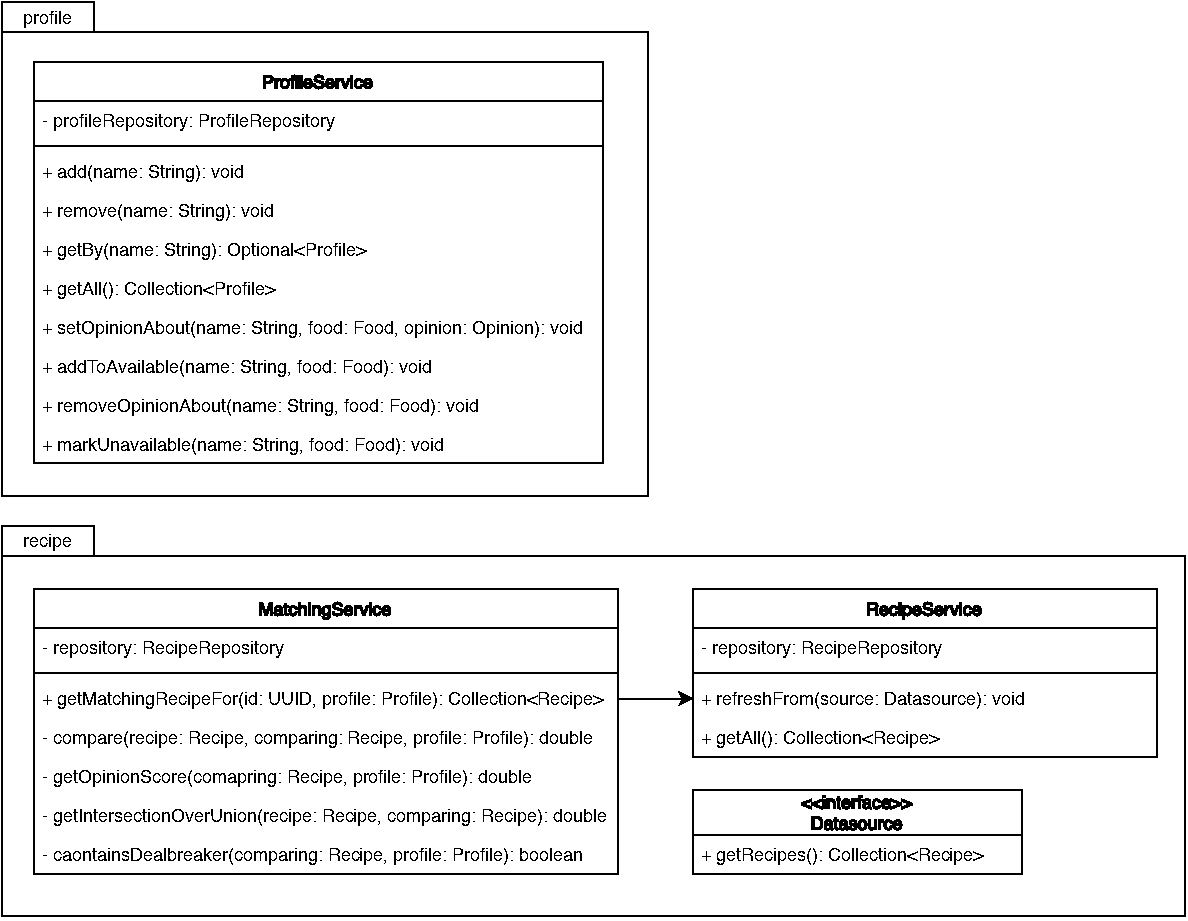
\includegraphics[width=0.98\columnwidth]{../diagrams/application_uml.pdf}
    \caption{Klassendiagramm der Applikationsschicht}
    \label{fig:class-diag-application}
\end{figure}

Die einzige Abhängigkeit des Modules besteht dabei auf den Domaincode der Software.

\section{Schicht 1: Adapters}
Die Adapterschicht wurde im Module \code{1-quickie-adapters} implementiert und erfüllt in der zugrundeliegenden Software zwei Aufgaben: Zum einen werden die Daten durch Mapper-Klassen von dem Format, welches die Services aus der Applikationsschicht liefern, in das Format übersetzt, welches die Plugins benötigen und umgekehrt. Zum anderen regelt sie die Kommunikation zwischen den Plugins und der Applikationsschicht. Um hierbei eine möglichst große Entkopplung zwischen den Plugins und Applikationsschicht zu erreichen, geschieht diese Kommunikation eventbasiert.

\begin{figure}[ht!]
    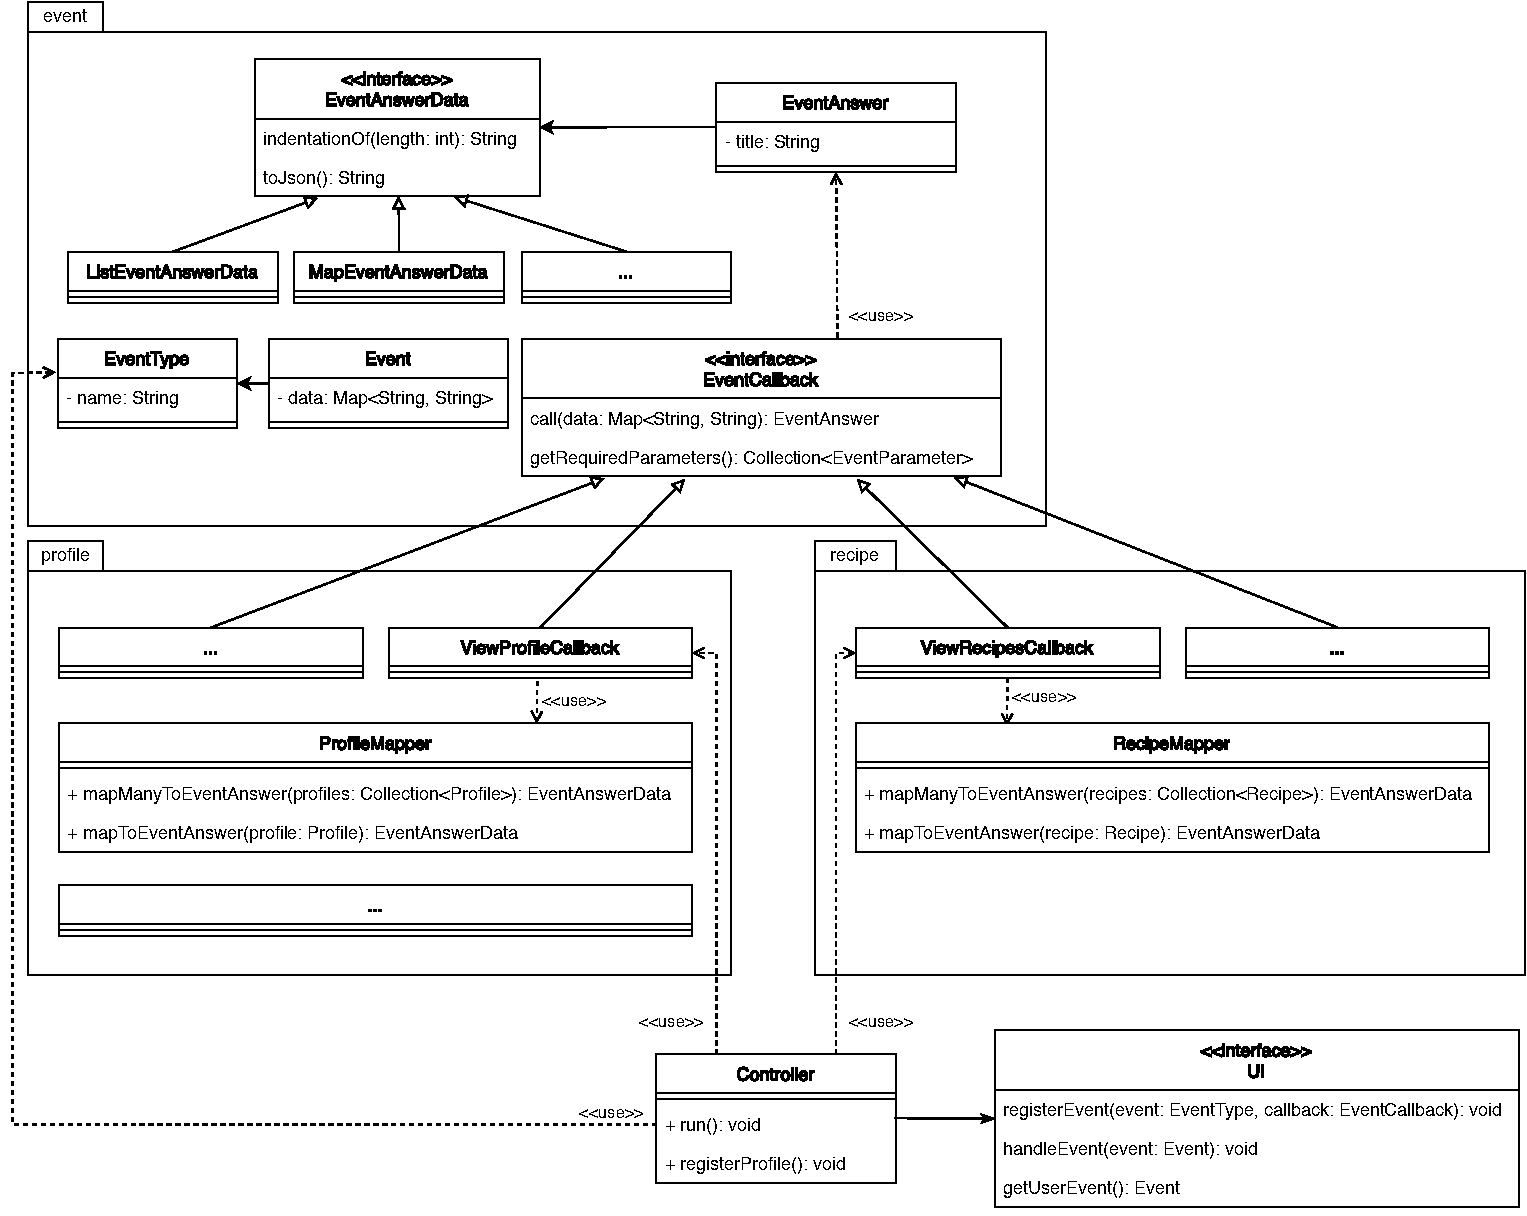
\includegraphics[width=0.98\columnwidth]{../diagrams/adapter_uml.pdf}
    \caption{Vereinfachter Ausschnitt des Klassendiagramms der Adapterschicht}
    \label{fig:class-diag-adapter}
\end{figure}

\autoref{fig:class-diag-adapter} zeigt einen Ausschnitt des Klassendiagramms der Adapterschicht in vereinfachter Form. Die Adapterschicht besitzt vier Packages: \code{event}, \code{profile}, \code{recipe} und \code{persistence}. Letzteres wurde hier im Sinne der Übersichtlichkeit zunächst nicht dargestellt. 

Das Package \code{event} enthält Pure Fabrication Code, welcher ausschließlich die eventbasierte Kommunikation betrifft. Die Klasse \code{Event} repräsentiert hierbei ein Event, welches von der Benutzeroberfläche gesendet wird und besitzt einen \code{EventType}. Die Klasse \code{EventAnswer} bildet das Resultat der Verarbeitung eines Events ab, welches an die Benutzeroberfläche zurückgeschickt wird. Die Daten, welche mittels der \code{EventAnswer} an die Benutzeroberfläche geschickt werden, werden in einem separaten Objekt gehalten. Hierbei handelt es sich je nach Form der Daten um eine Instanz einer Klasse, welche das Interface \code{EventAnswerData} implementiert. Die Logik, welche beim Auftreten eines bestimmten Events aufgerufen wird, befindet sich in Callback-Klassen. Zu jedem \code{EventType} existiert eine eine entsprechende Callback-Klasse, welche das Interface \code{EventCallback} implementiert.

In den Packages \code{profile} und \code{recipe} werden zum einen die entsprechenden Callback-Klassen implementiert und zum anderen Mapper-Klassen, welche die von der Applikationsschicht erhaltenen Daten in das von der Benutzeroberfläche benötigte Format überführen.

Das zentrale Element der Adapterschicht ist der Controller. Dieser registriert beim Start der Applikation zunächst für jeden \code{EventType} die zugehörige Callback-Klasse bei der Benutzeroberfläche, welche das Interface \code{UI} implementieren muss. Er bildet außerdem den Einstiegspunkt bei der Verarbeitung eines Events von der Benutzeroberfläche, indem er das aufgetretene Event von der Benutzeroberfläche abfragt und dessen Verarbeitung durch den Aufruf der Methode \code{handleEvent} in Gang setzt. 

\begin{figure}[ht!]
    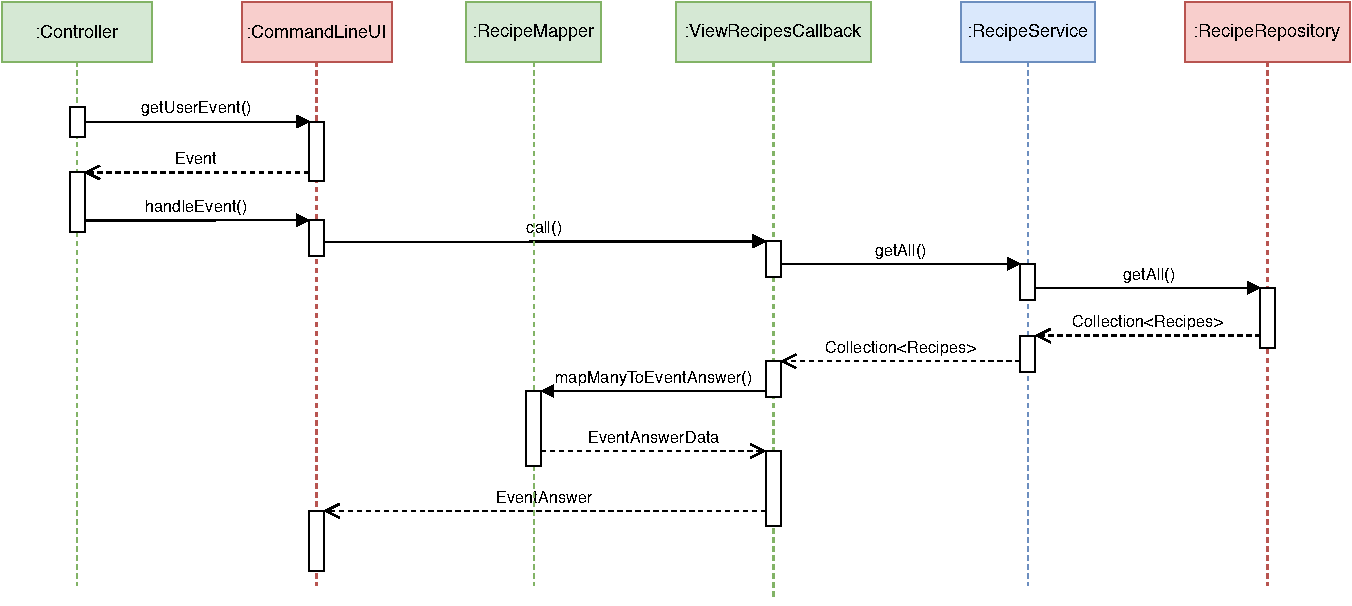
\includegraphics[width=0.98\columnwidth]{../diagrams/adapter_sequence.pdf}
    \caption{Verarbeitung eines User-Events}
    \label{fig:squence-diag-adapter}
\end{figure}

\autoref{fig:squence-diag-adapter} zeigt beispielhaft den Ablauf bei der Verarbeitung eines Events vom Typ \code{viewRecipes}. Die beteiligten Objekte sind hier farblich nach ihrer Schichtzugehörigkeit markiert: Grün steht für die Adapterschicht, Blau für die Applikationsschicht und Rot für ein Plugin.

Das Package \code{persistence} bildet die Schnittstelle zwischen der Applikationsschicht und Plugins für die Persistenz. Hier werden Interfaces definiert, welche die zu persistierenden Klassen implementieren müssen, nämlich \code{PersistentProfile}, \code{PersistentRecipe} und \code{PersistentIngredient}. Außerdem werden die Mapper-Klassen \code{PersistentProfileMapper} und \code{PersistenRecipeMapper} implementiert, welche die Domänenobjekte in ihre persistenten Gegenstücke transformieren und umgekehrt. Ferner werden in dem Package die Interfaces \code{PersistentProfileFactory} und \code{PersistentRecipeFactory} definiert, welche dann im Persistenz-Plugin implementiert werden und in den Mapper-Klassen verwendet werden, um leere \code{PersistentProfile}s und \code{PersistentRecipe}s zu erzeugen. Zuletzt werden hier auch die beiden im Domaincode definierten Interfaces \code{RecipeRepository} und \code{ProfileRepository} in den beiden abstrakten Klassen \code{PersitentRecipeRepository} und \code{PersistentProfileRepository} implementiert, von welchen dann die Repositories in einem Persistenz-Plugin erben.

\section{Schicht 0: Plugins}

\subsection{Plugin \acs{CLI}}
Dieses Plugin, welches im Module \code{0-quickie-plugin-cli} implementiert wurde und die Benutzeroberfläche der Software bildet, enthält lediglich die Klasse \code{CommandLineUI}. Diese implementiert das Interface \code{UI} aus der Adapterschicht. Abgesehen von dieser besitzt dieses Plugin nur eine weitere Abhängigkeit: Die Library Apache Commons \acs{CLI}, welche zur leichteren Implementierung der \ac{CLI} verwendet wird. Das Plugin kommuniziert lediglich über die Eventfunktionalität der Adapterschicht mit dem Kern der Software, ist damit nur sehr lose an den selben gekoppelt und kann leicht ausgetauscht werden.

\subsection{Plugin Gson}

\subsection{Plugin JPA}
Dieses Plugin wurde im Module \code{0-quickie-plugin-jpa} realisiert die Persistenz der Software mit Hilfe der \ac{JPA} und deren Implementierung Hibernate. Auch dieses Plugin besitzt nur eine Abhängigkeit auf die Adapterschicht, da hier die dort im Package \code{persistence} definierten Interfaces für Factories und die zu persistierenden Objekte Recipe, Ingredient und Profile implementiert werden. Letztere enthalten außerdem die \ac{JPA}-Annotationen. Ferner enthält das Plugin die Klassen \code{JPARecipeRepository} und \code{JPAProfileRepository}, welche von den beiden abstrakten Repository-Klassen aus der Adapterschicht erben. Schließlich enthält das Plugin noch den \code{PersistenceMananger}, einen Singleton, welcher den \code{EntityManager} von \code{JPA} für die Repositories liefert.

\subsection{Plugin Scraper}
In diesem Plugin wird die Extraktion der Rezepte aus den entsprechenden Webseiten im Module \code{0-quickie-plugin-scraper} implementiert. Hierzu werden die Webseiten zunächst durch den \code{CachedDownloader} heruntergeladen. Für das Parsen der Webseiten wird der \code{HensslerScraper} verwendet, welcher die Rezeptdaten aus dem HTML-Text extrahiert. Diese werden dann durch die \code{HensslerDatasource}, welche das in der Applikationsschicht definierte Interface \code{Datasource} implementiert, für die Applikationsschicht zugänglich gemacht. Die Daten durchlaufen damit nicht die Adapterschicht, da der Scraper die Daten problemlos direkt in dem von der Applikationsschicht benötigten Format liefern kann.
% Redet mit Adapterschicht
% Hat ganz schön viel Logik 

\subsection{Plugin Main}
Das Module \code{0-quickie-main} enthält lediglich die Main-Klasse der Applikation, welche alle nötigen Klassen instanziiert und ggf. injected. Zuletzt wird hier auch die Methode \code{run} des Controllers aus der Adapterschicht ausgeführt und somit die Verarbeitung von Events gestartet. Dieses Modul besitzt folglich Abhängigkeiten auf alle anderen Modules der Software und befindet sich daher in der äußersten Schicht.
% Begründung dass das ein Plugin ist
